% ----- Consignes exo 5 ----- %
\begin{td-exo}[Sur le problème de couplage maximum de poids maximum ou minimum: un début d'étude polyédrale sur le problème de couplage]\,\\ % 5 
	Soit \(E(S)\) l'ensemble des arêtes d'un ensemble \(S\).

	\begin{enumerate}
		\item Donner le programme linéaire en nombres entiers qui modélise le problème (version minimum et maximum).

		\item Donner les équations des contraintes pour le graphe donné par la figure~\ref{fig:dm1_ex05_f1} ci-dessous pour la version minimum.

		\vspace{2mm}
\ffigbox[\FBwidth]{%
\caption{\centering Cas pathologique}\label{fig:dm1_ex05_f1}
}{
    \fbox{
        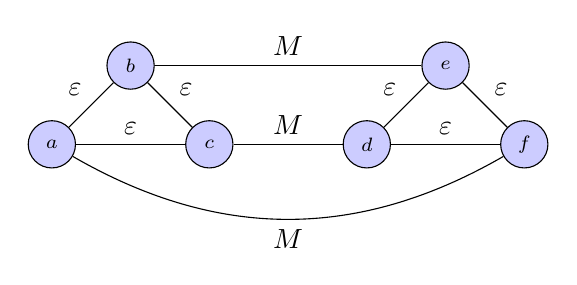
\begin{tikzpicture}[scale=1, main node/.style={circle, draw, fill=blue!20, inner sep=1pt, font=\scriptsize, minimum size=6mm, text=black}]
            % les sommets initiaux
            \node[main node] (1) at (0,0) {\(a\)};
            \node[main node] (2) at (1,1) {\(b\)};
            \node[main node] (3) at (2,0) {\(c\)};
            
            \node[main node] (4) at (4,0) {\(d\)};
            \node[main node] (5) at (5,1) {\(e\)};
            \node[main node] (6) at (6,0) {\(f\)};

            % aretes
            \draw (1) to node[above left] {\(\varepsilon\)} (2);
            \draw (1) to node[above] {\(\varepsilon\)} (3);
            \draw (2) to node[above right] {\(\varepsilon\)} (3);

            \draw (4) to node[above left] {\(\varepsilon\)} (5);
            \draw (4) to node[above] {\(\varepsilon\)} (6);
            \draw (5) to node[above right] {\(\varepsilon\)} (6);

            \draw (2) to node[above] {\(M\)} (5);
            \draw (3) to node[above] {\(M\)} (4);
            
            \draw[bend right] (1) to node[below] {\(M\)} (6);

        \end{tikzpicture}
    }
}

		\item Donner une solution optimale notée \(z(ILP)\) pour la figure~\ref{fig:dm1_ex05_f1}.

		\item Donner une solution pour le programme relaxé notée \(z(LP)\) pour la figure~\ref{fig:dm1_ex05_f1}.

		\item Conclure sur la pertinence de la formulation.

		\item Rajouter la condition 
		\begin{equation*}
			\forall S \subseteq V: |S| \text{ impair} \implies \sum_{e \in E(S)} x_e \leq \frac{|S|-1}{2}
		\end{equation*}
		et vérifier les équations sur l'exemple donné à la figure~\ref{fig:dm1_ex05_f1} sur un triangle.

		\item Donner une description sous forme de programme linéaire en nombres entiers du problème du couplage maximal de cardinalité minimum (CMCM). C'est à dire, on cherche un couplage maximal \(C\) tel que pour tout couplage maximal \(C'\), on ait \(|C| \leq |C'|\).

		\item Decrire un algorithme polynomial de \(2\)-approximation du problème du couplage maximal.

		\item Représentation du polytope du couplage. 
		
		Le vecteur caractéristique des couplages dans \(G\) peuvent être vu comme des points de \(\bb R^m\) avec \(m = |E|\). 
		Ainsi

		\begin{definition}
			Pour un graphe \(G\) donné, le polytope \(M\) du couplage est l'envelopppe convexe de tous les couplages dans \(G\).
			Ainsi
			\begin{equation*}
				M = \left\{ \sum_i \lambda_i M_i \ \mid\ \forall i, \lambda_i \geq 0,\ M_i \text{ est un couplage dans } G,\ \sum_i \lambda_i = 1 \right\}
			\end{equation*}
		\end{definition}
		\begin{definition}
			Pour un graphe \(G\) donné, le polytope fractionnaire \(FM\) du couplage est défini comme la région réalisable pour le programme relaxé l'enveloppe convexe de tous les couplages dans \(G\).
			Ainsi
			\begin{equation*}
				FM = \left\{ \sum_i \lambda_i M_i \ \mid\ \forall i, \lambda_i \geq 0,\ M_i \text{ est un couplage dans } G,\ \sum_i \lambda_i = 1 \right\}
			\end{equation*}
		\end{definition}
		La différence entre \(FM\) et \(M\) porte sur la relaxation des contraintes d'intégrité \(x_\varepsilon \in \ff{0, 1}\) à la place de \(x_\varepsilon \in \{0, 1\}\).

		On peut étendre ces définitions en prenant des couplages parfaits à la place des couplages en considérant \(PM\) et \(FPM\).

		\begin{enumerate}
			\item Pour les graphes donnés par la figure~\ref{fig:dm1_ex05_f2} ci-dessous, donner pour chacun l'ensemble des points possibles pour le programme linéaire en nombres entiers et le polytope du couplage \(M\) associé.

			\vspace{2mm}
\ffigbox[\FBwidth]{%
\caption{\centering Ensemble de graphes}\label{fig:dm1_ex05_f2}
}{
    \fbox{

    \begin{subfigure}{68.68655pt}
    \centering
    \fbox{
    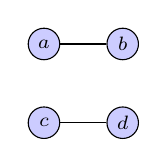
\begin{tikzpicture}[scale=1, main node/.style={circle, draw, fill=blue!20, inner sep=1pt, font=\scriptsize, minimum size=4mm, text=black}]
        \node[main node] (1) at (0,0) {\(a\)};
        \node[main node] (2) at (1,0) {\(b\)};
        \node[main node] (3) at (0,-1) {\(c\)};
        \node[main node] (4) at (1,-1) {\(d\)};
        \draw (1) -- (2);
        \draw (3) -- (4);
    \end{tikzpicture}
    }
    \caption{Un couplage}\label{fig:dm1_ex05_f2_sub1} 
    \end{subfigure}

    \begin{subfigure}{68.68655pt}
    \centering
    \fbox{
    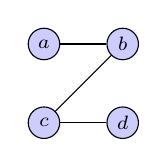
\begin{tikzpicture}[scale=1, main node/.style={circle, draw, fill=blue!20, inner sep=1pt, font=\scriptsize, minimum size=4mm, text=black}]
        \node[main node] (1) at (0,0) {\(a\)};
        \node[main node] (2) at (1,0) {\(b\)};
        \node[main node] (3) at (0,-1) {\(c\)};
        \node[main node] (4) at (1,-1) {\(d\)};
        \draw (1) -- (2);
        \draw (2) -- (3);
        \draw (3) -- (4);
    \end{tikzpicture}
    }
    \caption{Un chemin}\label{fig:dm1_ex05_f2_sub2} % chktex 10
    \end{subfigure}

    \begin{subfigure}{94.58174pt}
    \centering
    \fbox{
    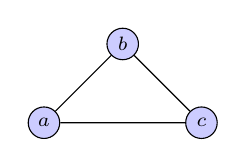
\begin{tikzpicture}[scale=1, main node/.style={circle, draw, fill=blue!20, inner sep=1pt, font=\scriptsize, minimum size=4mm, text=black}]
        \node[main node] (1) at (0,0) {\(a\)};
        \node[main node] (2) at (1,1) {\(b\)};
        \node[main node] (3) at (2,0) {\(c\)};
        \draw (1) -- (2) -- (3) -- (1);
    \end{tikzpicture}
    }
    \caption{Un triangle}\label{fig:dm1_ex05_f2_sub3} % chktex 10
    \end{subfigure}
    }
    
} % chktex 10 chktex 17

			\item Montrer les propositions suivantes:

			\begin{enumerate}
				\item \(M \subseteq FM\),

				\item Si \(G\) est biparti alors \(M = FM\).
				Pour cela procédons par contradiction.
				Supposons que \(x\) soit un sommet non entier.
				Définissions \(G_x = (V, E_x)\) où \(E_x = \{e \in E \mid x_e \notin \{0, 1\}\}\).

				\begin{itemize}
					\item Supposons que \(G_x\) possède un cycle \(C\).
					Définir deux couplages \(x^+\) et \(x^-\) obtenus à partir de \(x\) en supprimant et ajoutant un \(\varepsilon\) (à vous de le définir).
					\item Supposons que \(G_x\) ne possède pas de cycle.
					Définir deux couplages \(x^+\) et \(x^-\) obtenus à partir de \(x\) en supprimant et ajoutant un \(\varepsilon\) (à vous de le définir).
				\end{itemize}

				\item Si \(G\) est non biparti, alors \(M \neq FM\).
			\end{enumerate}

			\item Dans le cas du triangle, positionner le point de coordonnées \(\left(\frac{1}{2}, \frac{1}{2}, \frac{1}{2}\right)\).
			Conclure sur son appartenance au polytope.
			Conclure sur le programme linéaire en nombres entiers donné ci-dessus.

			\item Montrer que pour les graphes bipartis, le programme relaxé donne un couplage comme une solution optimale.
			Pour cela, comparer les sommets du polytope du couplage fractionnaire et du polytope du couplage.
		\end{enumerate}
	\end{enumerate}
\end{td-exo}

% ----- Solutions exo 5 ----- %
\iftoggle{showsolutions}{ 
	\begin{td-sol}[]\ % 5
		\begin{enumerate}
			\item Le programme linéaire se fait en deux temps étant donné qu'on a deux objectifs à atteindre.
			Dans un premier temps on cherche à maximiser la taille du couplage:
			\begin{equation*}
				\begin{cases}
					\max \sum_{e \in E} x_e \\
					\sum_{e \in \delta(v)} x_e \leq 1 \quad \forall v \in V \\
					x_e \in \{0, 1\} \quad \forall e \in E
				\end{cases}
			\end{equation*}
			Cette formulation correspond à 
			\begin{itemize}
				\item Maximiser le nombre d'arêtes sélectionnées dans le couplage.
				\item La première contrainte garantit que chaque sommet est incident à au plus une arête du couplage, ce qui est la définition d'un couplage.
				\item La deuxième contrainte impose que les variables \(x_e\) soient binaires, c'est-à-dire que chaque arête soit soit sélectionnée (1) soit non sélectionnée (0).
			\end{itemize}
			Ensuite, on cherche à minimiser le poids du couplage maximal:
			\begin{equation*}
				\begin{cases}
					\min \sum_{e \in E} w_e x_e \\
					\sum_{e \in E} x_e = k \\
					\sum_{e \in \delta(v)} x_e \leq 1 \quad \forall v \in V \\
					x_e \in \{0, 1\} \quad \forall e \in E
				\end{cases}
			\end{equation*}
			où \(k\) est la taille maximale du couplage trouvée dans la première étape.
			Cette formulation correspond à
			\begin{itemize}
				\item Minimiser le poids total du couplage sélectionné.
				\item La première contrainte garantit que le couplage sélectionné a exactement \(k\) arêtes, ce qui correspond à la taille maximale du couplage trouvée précédemment.
				\item La deuxième contrainte garantit que chaque sommet est incident à au plus une arête du couplage, ce qui est la définition d'un couplage.
				\item La troisième contrainte impose que les variables \(x_e\) soient binaires, c'est-à-dire que chaque arête soit soit sélectionnée (1) soit non sélectionnée (0).
			\end{itemize}

			Pour combiner ces deux formulations on peut s'aider d'une constante \(M\) suffisamment grande pour garantir que la minimisation du poids ne prenne pas le pas sur la maximisation de la taille du couplage:
			\begin{equation*}
				\begin{cases}
					\min \sum_{e \in E} w_e x_e - M \sum_{e \in E} x_e \\
					\sum_{e \in \delta(v)} x_e \leq 1 \quad \forall v \in V \\
					x_e \in \{0, 1\} \quad \forall e \in E
				\end{cases}
			\end{equation*}
			Cette formulation correspond à
			\begin{itemize}
				\item Minimiser le poids total du couplage sélectionné tout en maximisant la taille du couplage grâce à la constante \(M\) qui pénalise fortement les solutions de petite taille.
				\item La première contrainte garantit que chaque sommet est incident à au plus une arête du couplage, ce qui est la définition d'un couplage.
				\item La deuxième contrainte impose que les variables \(x_e\) soient binaires, c'est-à-dire que chaque arête soit soit sélectionnée (1) soit non sélectionnée (0).
			\end{itemize}
			Ici on peut prendre \(M = \sum_{e \in E} w_e + 1\) pour garantir que la maximisation de la taille du couplage soit prioritaire sur la minimisation du poids.

			Pour la version maximum, il suffit de remplacer la fonction objectif par \(\max \sum_{e \in E} w_e x_e + M \sum_{e \in E} x_e\) pour maximiser à la fois le poids et la taille du couplage (à noter qu'ici on peut se passer de la constante \(M\) car on cherche à maximiser les deux objectifs, mais cela peut être utile pour garantir que la maximisation de la taille du couplage soit prioritaire sur la maximisation du poids).

			\item Les équations des contraintes pour la figure~\ref{fig:dm1_ex05_f1} sont les suivantes:
			\begin{equation*}
				\begin{cases}
					\min \left(\varepsilon \cdot \left(ab + ac + bc + de + df + ef\right) + M \cdot \left(af + be + cd\right)\right)\\
					\sum_{e\in E} x_e = 3 \\
					x_{ab} + x_{ac} + x_{af} \leq 1 \\
					x_{ab} + x_{bc} + x_{be} \leq 1 \\
					x_{ac} + x_{bc} + x_{cd} \leq 1 \\
					x_{cd} + x_{de} + x_{df} \leq 1 \\
					x_{be} + x_{de} + x_{ef} \leq 1 \\
					x_{af} + x_{df} + x_{ef} \leq 1 \\
					x_e \in \{0, 1\} \quad \forall e \in E
				\end{cases}
			\end{equation*}
			où \(x_{ij}\) représente la variable binaire associée à l'arête entre les sommets \(i\) et \(j\).

			\item Une solution optimale pour la figure~\ref{fig:dm1_ex05_f1} est donnée par le couplage \(\{ab, cd, ef\}\) qui a une taille de \(3\) et un poids de \(2 \varepsilon + M\).

			\item Une solution pour le programme relaxé est donnée par le couplage fractionnaire où \(x_{ab} = x_{ac} = x_{bc} = x_{de} = x_{df} = x_{ef} = \frac{1}{2}\) et \(x_{af} = x_{be} = x_{cd} = 0\) qui a une taille de \(3\) (6 arêtes à \(1/2\)) et un poids de \(\frac{1}{2} \cdot \varepsilon \cdot 6 = 3 \varepsilon\).

			\item On peut en conclure que la formulation (ILP) permet de donner une solution optimale pour le problème du couplage maximum de poids minimum, tandis que la formulation relaxée (LP) ne permet pas de garantir une solution optimale, car elle peut donner des solutions fractionnaires qui ne correspondent pas à des couplages valides dans le graphe.
			La contrainte d'intégrité \(x_e \in \{0, 1\}\) est donc essentielle pour garantir que les solutions obtenues correspondent à des couplages valides, tandis que la relaxation de cette contrainte peut conduire à des solutions qui ne sont pas réalisables dans le contexte du problème du couplage.
			En particulier, dans le cas de la figure~\ref{fig:dm1_ex05_f1}, la solution relaxée donne un poids de \(3 \varepsilon\) qui est inférieur au poids de la solution optimale \(2 \varepsilon + M\), ce qui montre que la solution relaxée n'est même pas solution réalisable.

			\item En rajoutant la condition
			\begin{equation*}
				\forall S \subseteq V: |S| \text{ impair} \implies \sum_{e \in E(S)} x_e \leq \frac{|S|-1}{2}
			\end{equation*}
			notre formulation devient
			\begin{equation*}
				\begin{cases}
					\min \sum_{e \in E} w_e x_e - M \sum_{e \in E} x_e \\
					\sum_{e \in \delta(v)} x_e \leq 1 \quad \forall v \in V \\
					\forall S \subseteq V: |S| \text{ impair} \implies \sum_{e \in E(S)} x_e \leq \frac{|S|-1}{2} \\
					x_e \in \{0, 1\} \quad \forall e \in E
				\end{cases}
			\end{equation*}
			On peut appliquer cette contrainte sur le triangle formé par les sommets \(a\), \(b\) et \(c\) de la figure~\ref{fig:dm1_ex05_f1}.
			Pour le triangle \(S = \{a, b, c\}\), on a \(E(S) = \{ab, ac, bc\}\) et \(|S| = 3\) qui est impair, donc la contrainte devient
			\begin{equation*}
				x_{ab} + x_{ac} + x_{bc} \leq \frac{3-1}{2} = 1
			\end{equation*}
			Cette contrainte est vérifiée par la solution optimale \(x_{ab} = 1\), \(x_{ac} = 0\) et \(x_{bc} = 0\) qui correspond au couplage \(\{ab, cd, ef\}\) et qui a un poids de \(2 \varepsilon + M\).
			En revanche, la solution relaxée \(x_{ab} = x_{ac} = x_{bc} = \frac{1}{2}\) ne vérifie pas cette contrainte, car \(x_{ab} + x_{ac} + x_{bc} = \frac{1}{2} + \frac{1}{2} + \frac{1}{2} = \frac{3}{2} > 1\).
			Cette contrainte permet donc de forcer la solution relaxée à respecter les propriétés d'un couplage valide, ce qui peut aider à rapprocher la solution relaxée de la solution optimale du programme linéaire en nombres entiers.
			
			On peut voir cette contrainte comme ``tout triangle ne peut contenir au plus qu'une arête du couplage maximum''.
		\end{enumerate}
	\end{td-sol}
}{}
